% TRACE-IDS report — standard IEEE two-column format.
% Overleaf: New Project -> Upload Project (zip this folder), OR paste this file into a blank
% project and upload report/figures/fewshot.png and report/figures/shap_importance.png.
% IEEEtran is built into Overleaf; no install needed.
%
% GUARDRAILS: numbers below come from results/metrics.csv and results/fewshot.csv (generated by
% src/evaluate.py and src/fewshot.py). Regenerate and update if the pipeline changes.
% Verify every \cite link opens before you compile.
\documentclass[conference]{IEEEtran}
\usepackage[T1]{fontenc}
\usepackage[utf8]{inputenc}
\usepackage{graphicx}
\usepackage{booktabs}
\graphicspath{{figures/}}

\begin{document}

\title{TRACE-IDS: Zero-Shot Cross-Dataset Intrusion Detection Fails,\\and Few-Shot Labeling Recovers It}
\author{\IEEEauthorblockN{Rijan Rayamajhi}
\IEEEauthorblockA{Independent Researcher\\ rayamajhirijan5051@gmail.com}}
\maketitle

\begin{abstract}
Machine-learning intrusion detectors reach near-perfect scores when trained and tested on one
dataset, but deployment means running on a network the model never saw. We evaluate this transfer
directly on two standardized NetFlow v3 datasets (NF-CICIDS2018 and NF-UNSW-NB15, 47 shared
features). Zero-shot transfer fails completely: a Random Forest with 0.95 in-dataset F1 detects
\emph{zero} attacks on the other dataset (cross-dataset recall 0.00), and its 0.96 ``accuracy'' is
an artifact of class imbalance. Per-dataset feature alignment, balanced class weights, and
explanation-guided feature selection do not fix it. The practical fix is cheap supervision: adding
only five labeled examples per class from the target network recovers 0.88 attack recall, ten give
0.93, and fifty give 0.99. Cross-dataset detection therefore needs a small, recurring amount of
target labeling for each new network, and we quantify how little.
\end{abstract}

\begin{IEEEkeywords}
intrusion detection, cross-dataset generalization, few-shot learning, transfer learning, NetFlow
\end{IEEEkeywords}

\section{Introduction}
Most machine-learning intrusion detectors are judged on one dataset: train on it, test on it,
report F1 above 0.95. Deployment is not like that. A real detector meets traffic from a network it
never trained on. We test that directly and find the benchmark numbers do not survive it: a Random
Forest trained on NF-CICIDS2018 scores 0.95 F1 in-dataset, then catches \emph{zero} attacks on
NF-UNSW-NB15.

The usual repairs do not help. Rescaling each dataset to a common range, weighting the minority
class, and selecting ``transferable'' features by SHAP all leave cross-dataset recall at zero. What
does help is a little target data: a handful of labeled flows from the new network restores most of
the detection. We measure how many are needed.

\begin{itemize}
\item On standardized NetFlow v3 data we show zero-shot cross-dataset detection fails outright
(recall 0.00), and that accuracy hides this because the target is 96\% benign.
\item We show alignment, balanced weights, and invariant-feature selection do not recover it.
\item We quantify a cheap fix: five labeled examples per class give 0.88 recall, ten give 0.93,
fifty give 0.99, so deployment on a new network needs very little labeling.
\end{itemize}

\section{Related Work}
Cross-dataset generalization of ML-NIDS is known to be poor: within-dataset scores above 0.95 fall
toward chance across datasets \cite{crossdataset}. Domain-invariant representation methods aim to
close this gap \cite{dinids}, and SHAP has been used to study feature transfer \cite{shapfs}.
Few-shot learning is the emerging practical direction, recovering strong cross-domain accuracy from
a handful of target samples \cite{fewshot}. We contribute a clean, reproducible measurement on
standardized NetFlow v3 data: the zero-shot failure, the fact that common fixes do not help, and a
few-shot recovery curve.

\section{Method}
\subsection{Datasets}
We use NF-CICIDS2018-v3 and NF-UNSW-NB15-v3. Both share one standardized 55-column NetFlow schema,
so no manual feature mapping is needed. We drop identifier columns (IP addresses, ports,
timestamps, attack-category) that leak dataset identity, keeping 47 flow-statistic features and the
binary label. NF-CICIDS2018 is subsampled to about 2M flows for tractability; NF-UNSW-NB15 is used
in full (about 2.2M flows). The datasets are imbalanced: 13\% attacks in CIC, 4\% in UNSW.

\subsection{Zero-Shot Transfer and the Fixes We Tried}
A Random Forest (200 trees, fixed seed, balanced class weights) trains on 70\% of CIC and is tested
on the held-out 30\% (same-dataset) and on all of UNSW (cross-dataset). We compare raw features
against per-dataset alignment (z-scoring each dataset by its own statistics), and against
explanation-guided invariant-feature selection (keep features important in both datasets with the
same effect direction, by SHAP). Because the target is heavily imbalanced, we report recall and F1,
not accuracy.

\subsection{Few-Shot Recovery}
We then add $k$ labeled flows per class, drawn from a target pool, to the source training set and
retrain, evaluating on a fixed held-out target test set. $k=0$ is zero-shot. Both datasets are
z-scored by their own statistics so they share a comparable space.

\section{Results and Discussion}
Table~\ref{tab:cross} shows the zero-shot picture. In-dataset F1 is 0.95, but cross-dataset recall
is 0.00 for every configuration: the detector labels all UNSW traffic benign and catches no attacks.
Its 0.96 cross-dataset ``accuracy'' is purely the benign fraction. Alignment changes nothing,
balanced weights do not rescue recall, and invariant-feature selection only lowers accuracy without
raising recall. On standardized features, naive transfer simply does not work.

\begin{table}[t]
\caption{Zero-shot transfer, NF-CICIDS2018 $\rightarrow$ NF-UNSW-NB15. Recall is attack detection.}
\label{tab:cross}
\centering
\begin{tabular}{lcccc}
\toprule
Configuration & same F1 & cross recall & cross F1 & cross acc \\
\midrule
No alignment (raw)              & 0.95 & 0.00 & 0.00 & 0.96 \\
Per-dataset alignment           & 0.95 & 0.00 & 0.00 & 0.96 \\
Alignment + invariant selection & 0.93 & 0.00 & 0.00 & 0.29 \\
\bottomrule
\end{tabular}
\end{table}

Figure~\ref{fig:fewshot} shows the fix. Adding just five labeled examples per class from the target
network raises attack recall from 0.00 to 0.88; ten give 0.93, fifty give 0.99. Detection recovers
almost completely with a trivial amount of target labeling.

\begin{figure}[t]
\centering
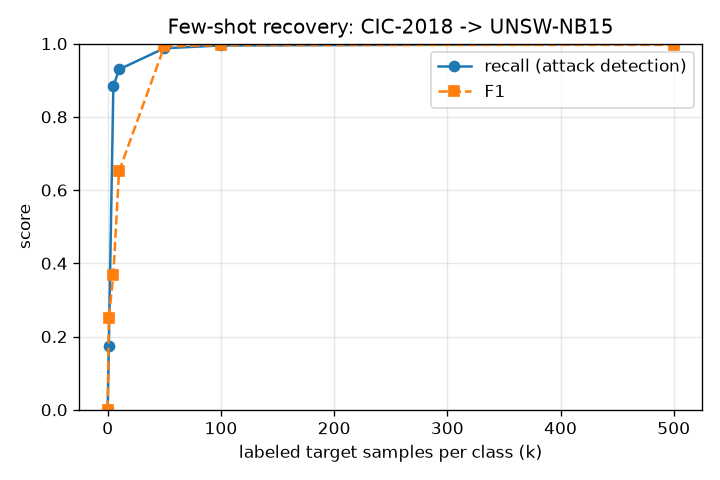
\includegraphics[width=\columnwidth]{fewshot.png}
\caption{Few-shot recovery. Zero-shot recall is 0.00; a handful of labeled target flows per class
restores detection (five $\rightarrow$ 0.88, ten $\rightarrow$ 0.93, fifty $\rightarrow$ 0.99).}
\label{fig:fewshot}
\end{figure}

\begin{figure}[t]
\centering
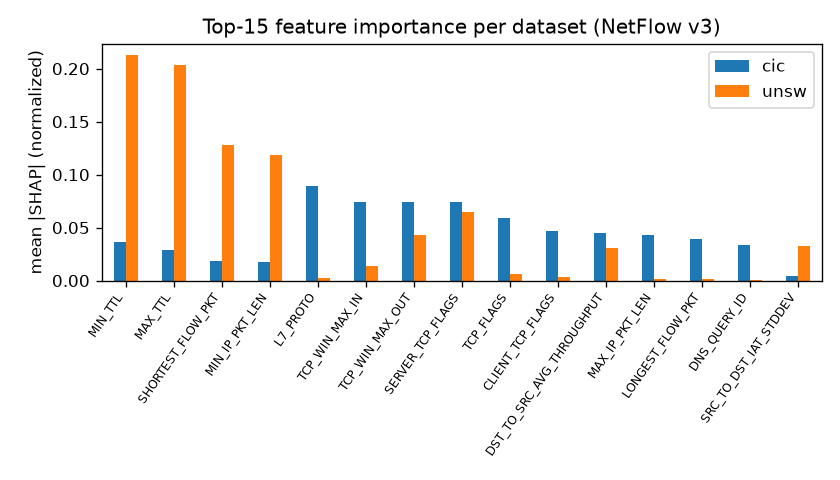
\includegraphics[width=\columnwidth]{shap_importance.png}
\caption{Per-dataset SHAP feature importance. The features the model leans on differ between
datasets, which is why a source-only model does not transfer.}
\label{fig:shap}
\end{figure}

The takeaway is practical. Attack signatures differ too much between networks for a source-only
model to reuse (Fig.~\ref{fig:shap}), so some target labeling is unavoidable. Full relabeling is
not: a few labeled flows per class on the new network are enough to redeploy a working detector.

\section{Conclusion}
On standardized NetFlow v3 data, zero-shot cross-dataset intrusion detection fails completely, and
feature alignment, balanced weights, and invariant-feature selection do not fix it. Few-shot
labeling does: five to fifty labeled examples per class recover 0.88 to 0.99 attack recall. The
study is limited to two datasets and a Random Forest; offline, no real-time or adversarial testing.
Future work: extend to a leave-one-dataset-out benchmark across more NetFlow datasets, and test
few-shot with deeper models.

\begin{thebibliography}{9}
% Verified 2026-10-06 (titles, authors, links confirmed), except [4] — verify author list before submitting.
\bibitem{crossdataset} M. Cantone, C. Marrocco, and A. Bria, ``On the Cross-Dataset Generalization of
Machine Learning for Network Intrusion Detection,'' \emph{IEEE Access}, vol.~12, 2024. arXiv:2402.10974.
\bibitem{dinids} S. Layeghy, M. Baktashmotlagh, and M. Portmann, ``DI-NIDS: Domain Invariant Network
Intrusion Detection System,'' 2022. arXiv:2210.08252.
\bibitem{shapfs} C. Kılıç and G. Şengül, ``SHAP-Guided Feature Selection for Cross-Dataset
Generalization in Network Intrusion Detection Systems,'' Atılım University, 2026.
\bibitem{fewshot} ``Few-shot network intrusion detection method based on multi-domain fusion and
cross-attention,'' \emph{PLOS ONE}, 2025. [verify authors before submitting]
\end{thebibliography}

\end{document}
